\section{Pflichtenheft}
	\SecAuth{\emplLastA, \emplLastC} % festlegen der Verfasser dieses Kapitels
	
\subsection{Git Integration}
s. https://tex.stackexchange.com/questions/261341/using-texstudio-and-git-to-automatically-commit-using-the-current-date

\begin{longlisting}
	\bashcode{src/commit.sh}
	\caption{script, um git commit durchzuführen}
\end{longlisting}

Einstellungen
\begin{figure}[h] % b... Grafik am Fuß, t... Grafik am Kopf, h... here
	\centering
	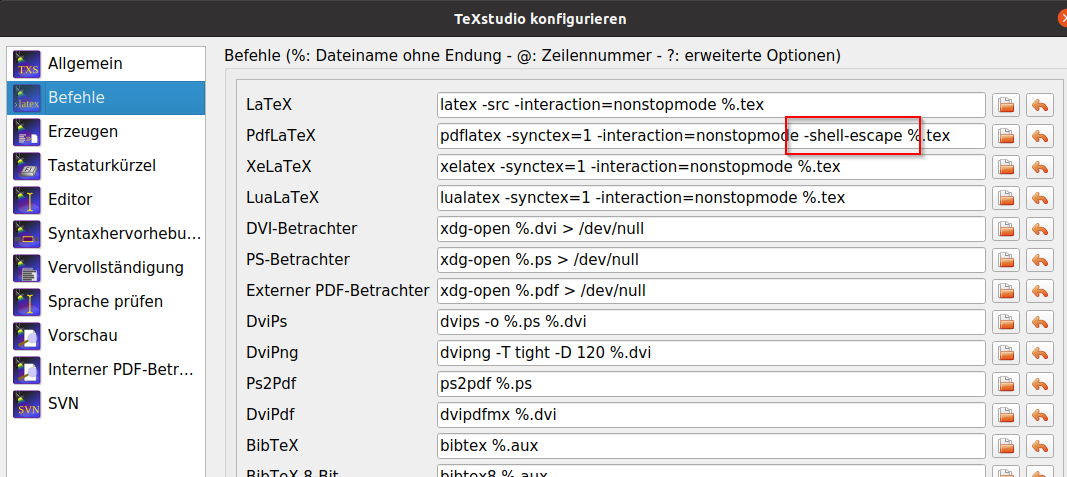
\includegraphics[width=0.6\linewidth]{chapter1/TeXstudio_Settings.png}
	\caption{TeXstudio Einstellungen}
\end{figure}

\begin{figure}[h] % b... Grafik am Fuß, t... Grafik am Kopf, h... here
\centering
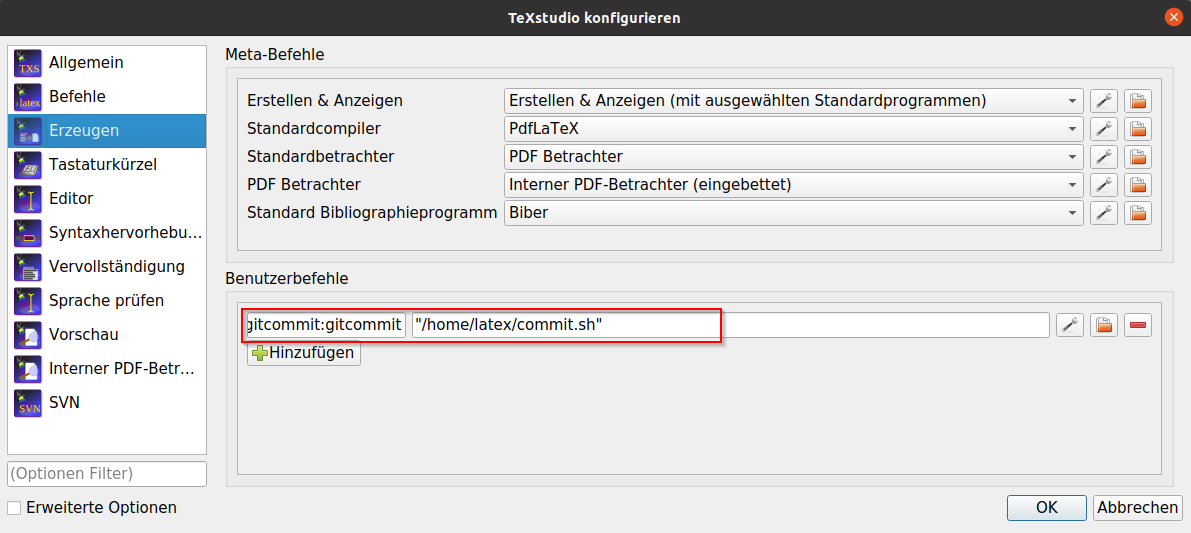
\includegraphics[width=0.6\linewidth]{chapter1/TeXstudio_AddCommand.png}
\caption{TeXstudio Befehl für commit einfügen}
\end{figure}

Commit kann jetzt mit Alt+Shift+F1 aufgerufen werden


\subsection{blabla}
\blindtext[1]

\subsubsection{blabla 1}
\blindtext[1]

\subsubsection{blabla 2}
\blindtext[1]

\pagebreak
